\documentclass[14pt]{article}
\usepackage[utf8]{inputenc}
\usepackage[T2A]{fontenc}
\usepackage[russian]{babel}
\usepackage{amsmath, amssymb}
\usepackage{geometry}
\usepackage{graphicx}
\usepackage{xcolor}
\usepackage{hyperref}
\usepackage{tasks}
\usepackage{tcolorbox}
\tcbuselibrary{skins, breakable, theorems}
\usepackage{fancyhdr}
\usepackage{lastpage}
\usepackage{enumitem}
\usepackage{paracol} % Для многоколоночности
\usepackage{ifthen}
\usepackage{needspace}

% Определение команд для тангенса и котангенса (русский стиль)
\newcommand{\tg}{\operatorname{tg}}
\newcommand{\ctg}{\operatorname{ctg}}

% Настройка геометрии для более компактного вида (как в мобильных приложениях)
\geometry{a4paper, left=10mm, right=10mm, top=20mm, bottom=20mm, headheight=15pt}

% Цветовая палитра (более современные и мягкие цвета)
\definecolor{primary}{RGB}{52, 152, 219}       % Ярко-синий
\definecolor{secondary}{RGB}{46, 204, 113}     % Зеленый
\definecolor{accent}{RGB}{155, 89, 182}        % Фиолетовый
\definecolor{lightbg}{RGB}{248, 249, 250}      % Светло-серый фон
\definecolor{taskborder}{RGB}{230, 230, 230}   % Цвет границы задач
\definecolor{optionbg}{RGB}{240, 242, 245}     % Фон для вариантов ответа

% Основной фон страницы
\pagecolor{lightbg}

% Настройка гиперссылок
\hypersetup{
    colorlinks=true,
    linkcolor=primary,
    urlcolor=primary,
}

% Колонтитулы (более стильные)
\pagestyle{fancy}
\fancyhf{}
\fancyhead[L]{\textcolor{primary}{\textbf{MathCore | MOCK Test-5}}}
\fancyhead[R]{\textcolor{secondary}{Abdunazarov M.X.}}
\fancyfoot[L]{\href{https://t.me/Math_Core_Dtm_MS_Att}{\textcolor{primary}{MathCore}}}
\fancyfoot[R]{\href{https://t.me/Abd_mardon}{\textcolor{secondary}{@Abd\_mardon}}}
\fancyfoot[C]{\textcolor{gray}{\thepage/\pageref{LastPage}}}
\renewcommand{\headrulewidth}{0.5pt}
\renewcommand{\headrule}{\hbox to\headwidth{\color{primary}\leaders\hrule height \headrulewidth\hfill}}
\renewcommand{\footrulewidth}{0.5pt}
\renewcommand{\footrule}{\hbox to\headwidth{\color{secondary}\leaders\hrule height \footrulewidth\hfill}}

% Титульная страница (улучшенная)
\title{\Huge \textbf{\textcolor{primary}{MOCK Test-5}}}
\author{\textcolor{secondary}{Abdunazarov M.X.}}
\date{}

% Стиль для карточки вопроса
\newtcolorbox{questionbox}[2][]{
    enhanced,
    breakable,
    colback=white,
    colframe=primary,
    coltitle=white,
    fonttitle=\bfseries\large,
    title={Задача \hfill \textcolor{white}{#2}},
    attach boxed title to top left={xshift=5mm, yshift=-2mm},
    boxed title style={size=small, colback=primary, sharp corners},
    sharp corners,
    boxrule=0.5pt,
    left=5mm,
    right=5mm,
    top=5mm,
    bottom=5mm,
    drop fuzzy shadow,
    #1
}

% Стиль для вариантов ответов (как кнопки)
\newlist{options}{enumerate}{1}
\setlist[options]{
    label=\textbf{\Alph*)},
    leftmargin=*,
    itemsep=2pt,
    topsep=5pt,
    before={\vspace{2mm}\begin{tcolorbox}[
        colback=optionbg,
        colframe=white,
        sharp corners,
        boxrule=0pt,
        left=2mm,
        right=2mm,
        top=2mm,
        bottom=2mm,
    ]},
    after={\end{tcolorbox}\vspace{2mm}},
}

% Для рисунков (центрирование и тень)
\newcommand{\questionimage}[2][0.5\linewidth]{%
    \begin{center}
        \includegraphics[width=#1]{#2}
    \end{center}
}

% Для удобства: команда вставки вопроса с рисунком
\newcommand{\questionitem}[4]{%
    \needspace{5cm} % Предотвращает разрыв вопроса
    \begin{questionbox}{#1}
        #2
        \ifx&#3&% Если рисунок не пустой
        \else
            \questionimage{#3}
        \fi
        \begin{options}
            #4
        \end{options}
    \end{questionbox}
}

\begin{document}

% Титульная страница
\maketitle
\begin{center}
    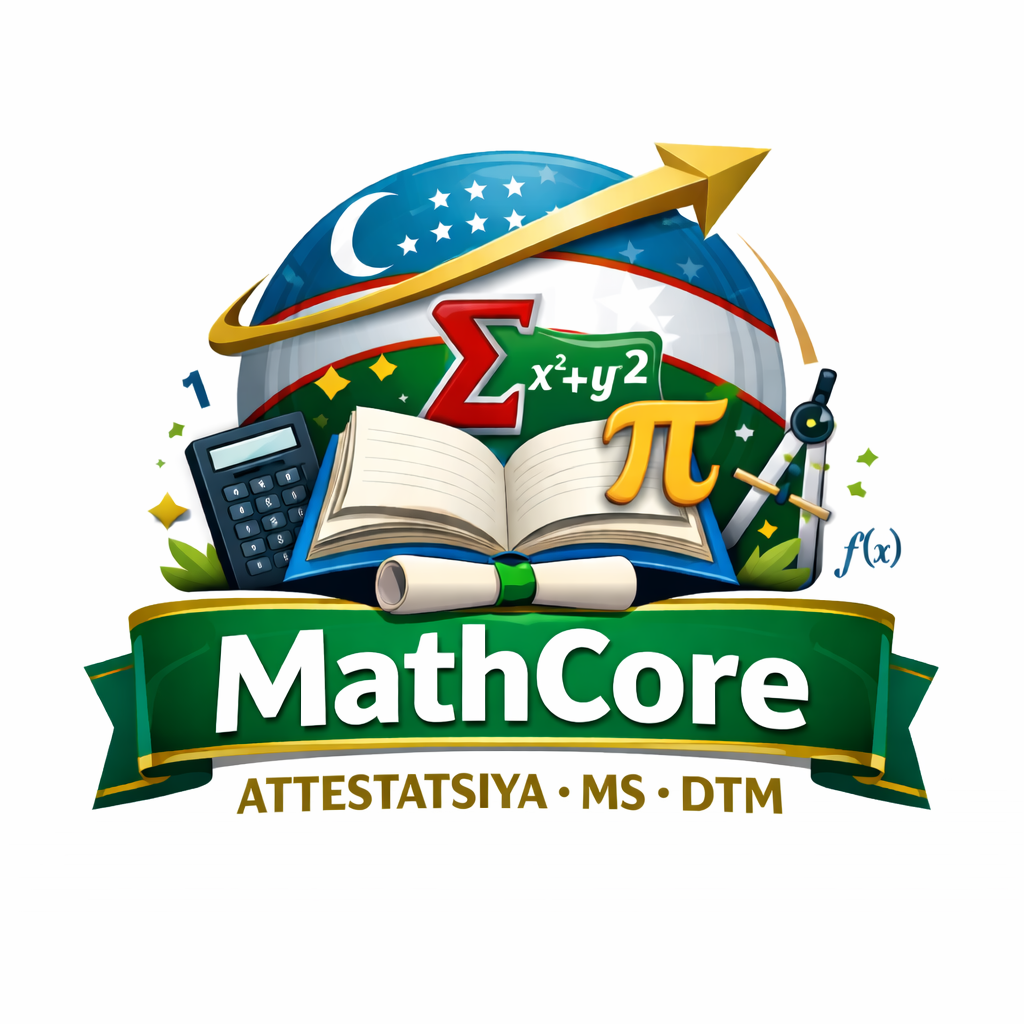
\includegraphics[width=0.2\textwidth]{logo.png} \\[5mm]
    \textcolor{gray}{\small Telegram: \href{https://t.me/Math_Core_Dtm_MS_Att}{@Math\_Core\_Dtm\_MS\_Att}}
\end{center}
\vspace{5mm}

% Двухколоночный режим для компактности
\columnratio{0.48,0.48}
\setlength{\columnsep}{0.04\textwidth}


% Задача 1
\begin{questionbox}{1}
    Если \( x^3 - 15^3 = 9^3 + 12^3 \), найдите \( x \).
    \begin{options}
        \item 21
        \item 28
        \item 20
        \item 18
    \end{options}
\end{questionbox}

% Задача 2
\begin{questionbox}{2}
    Вычислите \[\frac{1+2}{2} + \frac{1+2+3}{2^2} + \frac{1+2+3+4}{2^3} + \cdots\]
    \begin{options}
        \item \(\frac{28}{4}\)
        \item \(\frac{7}{2}\)
        \item \(\frac{7}{4}\)
        \item \(\frac{3}{2}\)
    \end{options}
\end{questionbox}

% Задача 3
\begin{questionbox}{3}
    Если числа \( x^2 + 5, \frac{1}{2} \sin \frac{\pi x}{4} \) и \(-4x\) являются последовательными членами арифметической прогрессии, сколько возможных значений может принимать \( x \)?
    \begin{options}
        \item 0
        \item 1
        \item 2
        \item 3
    \end{options}
\end{questionbox}

% Задача 4
\begin{questionbox}{4}
    К числителю несократимой дроби \(\frac{a}{b}\) прибавили 14, а к знаменателю 35, получив дробь \(\frac{c}{d}\). Если \( ad = bc \), найдите значение \( a + b \).
    \begin{options}
        \item 14
        \item 7
        \item 49
        \item невозможно определить
    \end{options}
\end{questionbox}

% Задача 5 (с рисунком)
\begin{questionbox}{5}
    На рисунке показаны \( n \) ступеней лестницы и расположенные на них красные и зеленые шары. Если общее количество шаров равно 210, сколько красных шаров?
    \questionimage{1.png}
    \begin{options}
        \item 105
        \item 110
        \item 112
        \item 115
    \end{options}
\end{questionbox}

% Задача 6
\begin{questionbox}{6}
    Если число \( n^n \) имеет 3001 цифру, сколько цифр в натуральном числе \( n \)?
    \begin{options}
        \item 2
        \item 3
        \item 4
        \item 5
    \end{options}
\end{questionbox}

% Задача 7
\begin{questionbox}{7}
    Первый сплав содержит 65\% золота и 35\% серебра. Второй сплав содержит 40\% золота и 60\% серебра. Сколько (кг) первого сплава нужно взять, чтобы получить 8 кг сплава, содержащего 50\% золота?
    \begin{options}
        \item 3,1(9)
        \item \(3\frac{2}{5}\)
        \item 4,8
        \item \(3\frac{2}{15}\)
    \end{options}
\end{questionbox}

% Задача 8
\begin{questionbox}{8}
    Функция \( f(x) = ax^2 + bx + c \) касается оси \( Ox \). Если уравнение оси симметрии \( x = 3 \), найдите значение \( \frac{c}{a} \).
    \begin{options}
        \item \(\frac{1}{9}\)
        \item 9
        \item \(-\frac{1}{9}\)
        \item невозможно определить
    \end{options}
\end{questionbox}

% Задача 9
\begin{questionbox}{9}
    Найдите остаток от деления числа \(-71\) на 6.
    \begin{options}
        \item \(-5\)
        \item 1
        \item 5
        \item \(-1\)
    \end{options}
\end{questionbox}

% Задача 10 (с рисунком)
\begin{questionbox}{10}
    На рисунке изображен график функции \( y = x^2 + nx + k \), наименьшее значение которой равно \(-1\). Используя данные на рисунке, найдите \( n + k \).
    \questionimage{2.png}
    \begin{options}
        \item 7
        \item 4
        \item 5
        \item 6
    \end{options}
\end{questionbox}

% Задача 11
\begin{questionbox}{11}
    На экзамене 36 вопросов: 21 сложный и 15 лёгких. Если известно, что первому вошедшему студенту достался сложный вопрос, найдите вероятность того, что четвёртому вошедшему достанется лёгкий вопрос.
    \begin{options}
        \item \(\frac{5}{12}\)
        \item \(\frac{1}{2}\)
        \item \(\frac{3}{7}\)
        \item 0,6
    \end{options}
\end{questionbox}

% Задача 12
\begin{questionbox}{12}
    Если $(x - 1)^3(2x - 1)^7 = a + a_1x + a_2x^2 + \cdots + a_{10}x^{10}$, найдите $a + a_1$.
    \begin{options}
        \item $-10$
        \item $-16$
        \item $-14$
        \item $-17$
    \end{options}
\end{questionbox}



% Задача 13
\begin{questionbox}{13}
    Если \( x_1, x_2 \) и \( x_3 \) являются корнями уравнения \( x^3 + 3x - 1 = 0 \), найдите значение выражения \( x_1x_2(x_1 + x_2) + x_1x_3(x_1 + x_3) + x_2x_3(x_2 + x_3) \).
    \begin{options}
        \item 0
        \item $-3$
        \item 1
        \item $-1$
    \end{options}
\end{questionbox}

% Задача 14
\begin{questionbox}{14}
    Если \( k = 2^{2022} \), найдите остаток от деления \( 7^{8k+3} \) на 15.
    \begin{options}
        \item 12
        \item 13
        \item 4
        \item 11
    \end{options}
\end{questionbox}

% Задача 15
\begin{questionbox}{15}
    Если \( a = \frac{\sqrt{3}(3+2\sqrt{3})}{4} \), найдите значение \( \frac{2}{1-\frac{2}{2+\frac{1}{a-2}}} \).
    \begin{options}
        \item \(3\sqrt{3}\)
        \item \(\frac{3\sqrt{3}+1}{2}\)
        \item \(3\sqrt{3} + 2\)
        \item \(\sqrt{3}\)
    \end{options}
\end{questionbox}

% Задача 16
\begin{questionbox}{16}
    Если \( ABCDA_1B_1C_1D_1 \) — куб, определите вектор, равный вектору \( A_1A - C_1D + BC \).
    \begin{options}
        \item \(BD\)
        \item \(B_1C\)
        \item \(B_1A_1\)
        \item \(AC\)
    \end{options}
\end{questionbox}

% Задача 17 (с рисунком)
\begin{questionbox}{17}
    На рисунке изображены графики функций \( y = x^2 + 2 \) и \( y = \frac{3}{x} \). Используя данные на рисунке, найдите площадь закрашенной области.
    \questionimage{3.png}
    \begin{options}
        \item \(\frac{1}{4}\)
        \item \(\frac{2}{3}\)
        \item \(\frac{4}{5}\)
        \item \(\frac{4}{3}\)
    \end{options}
\end{questionbox}

% Задача 18
\begin{questionbox}{18}
    В арифметической прогрессии \( a_{30} = 3 \) и \( a_{32} = 11 \). Найдите наименьшее значение суммы первых \( n \) членов прогрессии.
    \begin{options}
        \item \(-1647\)
        \item \(-1652\)
        \item \(-1653\)
        \item \(-1650\)
    \end{options}
\end{questionbox}

% Задача 19
\begin{questionbox}{19}
    Для нумерации страниц сборника тестов по математике Сардора Салахиддинова, начиная с 3-й страницы, потребовалось 3523 цифры. Сколько страниц в сборнике?
    \begin{options}
        \item 1158
        \item 1112
        \item 1113
        \item 1159
    \end{options}
\end{questionbox}

% Задача 20
\begin{questionbox}{20}
    В трех сосудах всего 18 литров воды. Если половину воды из первого сосуда перелить во второй, затем треть образовавшейся воды во втором сосуде перелить в третий, и затем четверть образовавшейся воды в третьем сосуде перелить в первый, то во всех сосудах воды станет поровну. Сколько литров воды было первоначально в каждом сосуде?
    \begin{options}
        \item 8; 5; 5
        \item 3; 7; 8
        \item 6; 6; 6
        \item 4; 8; 6
    \end{options}
\end{questionbox}

% Задача 21
\begin{questionbox}{21}
    Если \(\cos(4x - 10^\circ) = -\frac{\sqrt{3}}{2}\), найдите наименьшее натуральное значение \( x \) (в градусах).
    \begin{options}
        \item 25
        \item 30
        \item 40
        \item 45
    \end{options}
\end{questionbox}

% Задача 22 (с рисунком)
\begin{questionbox}{22}
    Сколько различных хорд можно провести, соединяя 5 точек на окружности?
    \begin{center}
        
\includegraphics[width=0.2\textwidth]{4.png}
    \end{center}
    \begin{options}
        \item 5
        \item 4
        \item 10
        \item 8
    \end{options}
\end{questionbox}

% Задача 23
\begin{questionbox}{23}
    Дана последовательность с общим членом \( a_n = \frac{(n-1)!}{n^2 - n} \). Найдите значение \( \frac{a_{n+1}}{a_n} \).
    \begin{options}
        \item \(\frac{n(n-1)}{n+1}\)
        \item \(\frac{n+1}{2n}\)
        \item \(\frac{n(n+2)}{2n+2}\)
        \item \(\frac{2n}{n-1}\)
    \end{options}
\end{questionbox}

% Задача 24
\begin{questionbox}{24}
    В ящике 4 черных и 5 белых шаров. Найдите вероятность того, что два случайно выбранных шара оба белые.
    \begin{options}
        \item \(\frac{5}{18}\)
        \item \(\frac{2}{9}\)
        \item \(\frac{1}{6}\)
        \item \(\frac{1}{3}\)
    \end{options}
\end{questionbox}

% Задача 25
\begin{questionbox}{25}
    В каком варианте показана показательная функция?
    \begin{options}
        \item \((3\sqrt{-2})^x\)
        \item \((-2)^x\)
        \item \(3^{-x}\)
        \item \(1^x\)
    \end{options}
\end{questionbox}

% Задача 26
\begin{questionbox}{26}
    Найдите наименьшее натуральное решение неравенства \( 4^{\sqrt{2x+5}} - 10 \cdot 2^{\sqrt{2x+5}} + 16 > 0 \).
    \begin{options}
        \item 2
        \item 3
        \item 1
        \item 4
    \end{options}
\end{questionbox}

% Задача 27 (с рисунком)
\begin{questionbox}{27}
    На рисунке изображен прямоугольный треугольник \( ABC \). Если \( AB = \log_{27} 16 \) и \( AC = \log_2 81 \), найдите площадь треугольника \( ABC \).
    \questionimage{5.png}
    \begin{options}
        \item \(\frac{16}{3}\)
        \item 4
        \item \(\frac{8}{3}\)
        \item 2
    \end{options}
\end{questionbox}

% Задача 28
\begin{questionbox}{28}
    Площадь квадрата ABCD равна 36, а сторона AB параллельна оси абсцисс. Если вершины A, B и C лежат на графиках \( y = \log_a x \), \( y = 2 \log_a x \) и \( y = 3 \log_a x \) соответственно, найдите значение \( a \).
    \begin{options}
        \item \(\sqrt[6]{3}\)
        \item \(\sqrt[3]{3}\)
        \item \(\sqrt[3]{6}\)
        \item \(\sqrt[6]{6}\)
    \end{options}
\end{questionbox}

% Задача 29
\begin{questionbox}{29}
    Два квадрата со стороной 1 наложены друг на друга. Затем один из квадратов повернут на 45° вокруг их общего центра симметрии. Найдите площадь образовавшейся фигуры.
    \begin{options}
        \item \(4 - 2\sqrt{2}\)
        \item \(4 - \sqrt{2}\)
        \item 1,2
        \item 2,5
    \end{options}
\end{questionbox}

% Задача 30 (с рисунком)
\begin{questionbox}{30}
    На рисунке изображен график функции \( y = 9 - x^2 \). Используя информацию, представленную на рисунке, найдите наибольшее значение площади прямоугольника ABCD.
    \questionimage{6.png}
    \begin{options}
        \item \(12\sqrt{3}\)
        \item \(9\sqrt{3}\)
        \item \(6\sqrt{3}\)
        \item 12
    \end{options}
\end{questionbox}

% Задача 31 (с рисунком)
\begin{questionbox}{31}
    $OP = 8$ см, $PA = 2$ см, $OB = 10$ см. Плоскость, параллельная основанию прямого конуса с центром $O$ и радиусом основания 10 см, пересекает его и образует усеченный конус с центром основания $P$ и радиусом 2 см. Соответственно, найдите площадь боковой поверхности усеченного конуса на рисунке.
    \questionimage{36.png}
    \begin{options}
        \item $36\sqrt{2}$
        \item $72\sqrt{2}$
        \item $84\sqrt{2}$
        \item $96\sqrt{2}$
    \end{options}
\end{questionbox}

% Задача 32 (с рисунком)
\begin{questionbox}{32}
    В цилиндрический сосуд с радиусом основания 8 дм и высотой 25 дм налито некоторое количество воды. Если $OH = 4\sqrt{2}$ дм, то сколько литров воды в сосуде? (Примите $\pi = 3$)
    \questionimage{37.png}
    \begin{options}
        \item 400
        \item 480
        \item 500
        \item 520
    \end{options}
\end{questionbox}

% Задача 33 (с рисунком)
\begin{questionbox}{33}
    Точка $O$ — центр тяжести квадратной прямой пирамиды. $TE = \sqrt{5}$ см, $AE = 2\sqrt{5}$ см, $AB = 6$ см. Муравей, находящийся в точке $O$ пирамиды, может добраться до точки $E$ по поверхности пирамиды кратчайшим путем. Какое это расстояние?
    \questionimage{38.png}
    \begin{options}
        \item $\sqrt{38}$
        \item $3\sqrt{5}$
        \item 7
        \item $5\sqrt{2}$
    \end{options}
\end{questionbox}

% Задача 34 (с рисунком)
\begin{questionbox}{34}
    $TK = 7$ см, $AK = 17$ см, $OB = 6$ см. Муравей, находящийся в точке $A$ этого прямого конуса, может перемещаться по поверхности конуса до точки $K$ кратчайшим путем. Сколько см он должен пройти?
    \questionimage{39.png}
    \begin{options}
        \item 25
        \item 26
        \item 27
        \item 28
    \end{options}
\end{questionbox}

% Задача 35
\begin{questionbox}{35}
    Объем тела, полученного вращением множества $A = \{(x,y): x \geq 0, x + y \geq 1, 4x + y \leq 4\}$ вокруг оси $y$ на 360°, равен:
    \begin{options}
        \item $\pi$
        \item $\frac{4}{3}\pi$
        \item $\frac{3}{2}\pi$
        \item $\frac{5}{3}\pi$
    \end{options}
\end{questionbox}



\end{document}